
% This LaTeX was auto-generated from MATLAB code.
% To make changes, update the MATLAB code and republish this document.

\documentclass{article}
\usepackage{graphicx}
\usepackage{color}

\sloppy
\definecolor{lightgray}{gray}{0.5}
\setlength{\parindent}{0pt}

\begin{document}

    
    
\subsection*{Contents}

\begin{itemize}
\setlength{\itemsep}{-1ex}
   \item Lowe’s scale-invariant interest point detection
   \item Feature extraction
   \item Appendix
   \item function H2to1 = computeH(p1,p2)
   \item function H = computeHessian(I)
   \item function PrincipalCurvature = computePrincipalCurvature(DoGPyramid)
   \item function [DoGPyramid, DoGLevels] = createDoGPyramid(GaussianPyramid, levels)
   \item function [GaussianPyramid] = createGaussianPyramid(im, sigma0, k, levels)
   \item function displayPyramid(pyrmid)
   \item function [locsDoG, GaussianPyramid] = DoGdetector(im, sigma0, k, levels, th\_contrast, th\_r)
   \item function locsDoG = getLocalExtrema(DoGPyramid, DoGLevels, PrincipalCurvature, th\_contrast, th\_r)
   \item function [matches] = matchInterestPoints(desc1, desc2, ratio)
   \item function h = plotInterestPoints(im, locs, po)
   \item function index = randIndex(maxIndex,len)
   \item function [f] = ransac( x,y,ransacCoef,funcFindF,funcDist )
   \item function bestH = ransacH(matches, locs1, locs2, nIter, tol)
\end{itemize}


\subsection*{Lowe’s scale-invariant interest point detection}

\begin{verbatim}
im = imread('building_1.jpg');
im = im2double((im));
\end{verbatim}
\begin{par}
Parameters for Difference of Gaussians
\end{par} \vspace{1em}
\begin{verbatim}
scales = [-1, 0, 1, 2, 3, 4];
K = sqrt(2);
sigma0 = 1;
th_c = 0.03;
th_r = 12;
\end{verbatim}
\begin{par}
Get the interest points and the Gaussian Pyramid used to compute it
\end{par} \vspace{1em}
\begin{verbatim}
[locs,GP] = DoGdetector(rgb2gray(im), sigma0, K, scales, th_c, th_r);
plotInterestPoints(im,locs)
drawnow()
\end{verbatim}

        \color{lightgray} \begin{verbatim}
ans = 

  Image with properties:

           CData: [751x1024x3 double]
    CDataMapping: 'direct'

  Use GET to show all properties

\end{verbatim} \color{black}
    
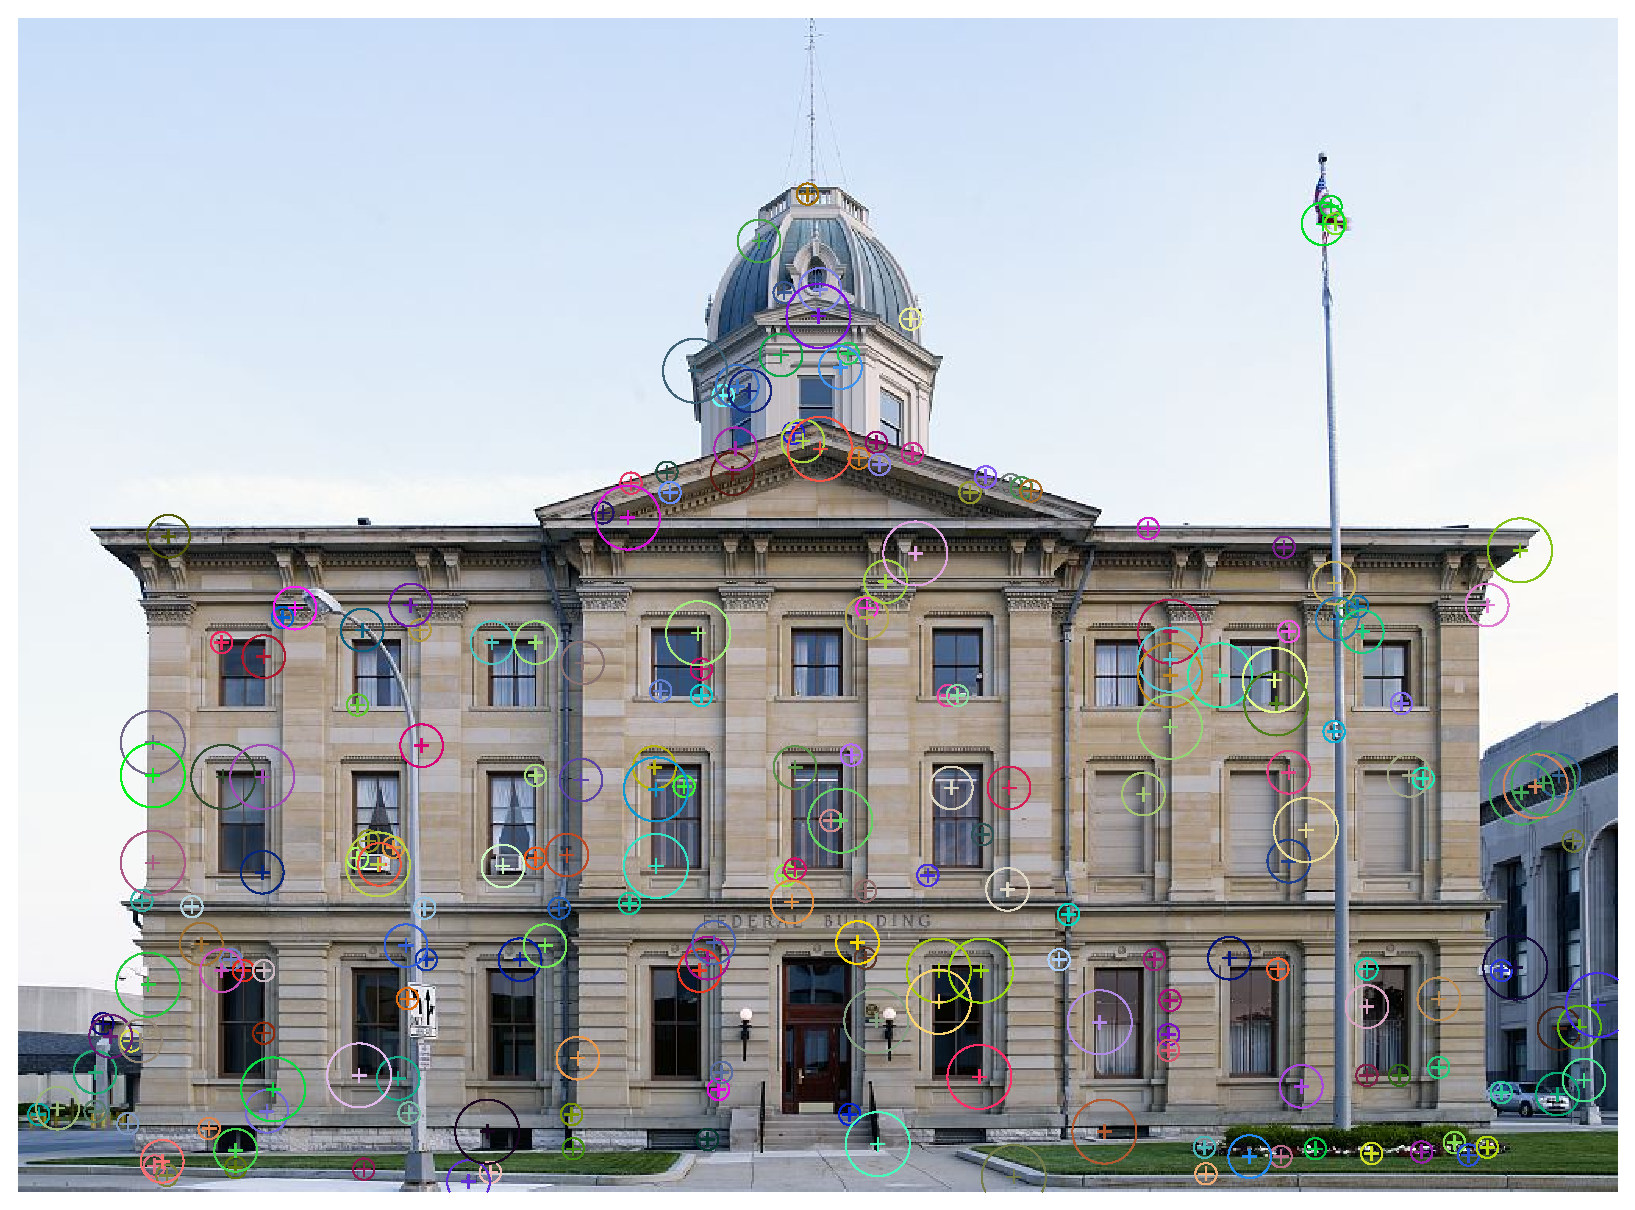
\includegraphics [width=4in]{debugScript_01.eps}
\begin{par}
Please look at the appendix for the code of individual functions
\end{par} \vspace{1em}


\subsection*{Feature extraction}

\begin{par}
Computed SIFT using vlfeat library
\end{par} \vspace{1em}
\begin{verbatim}
% addpath('/path/to/vlfeat')
im1 = imread('reference.png');
im2 = imread('test.png');
[locs1, desc1] = vl_sift(single(rgb2gray(im1)));
[locs2, desc2] = vl_sift(single(rgb2gray(im2)));
locs1 = locs1';
desc1 = desc1';
locs2 = locs2';
desc2 = desc2';
\end{verbatim}
\begin{par}
reference.png computed interest points
\end{par} \vspace{1em}
\begin{verbatim}
plotInterestPoints(im1, locs1);
drawnow()
\end{verbatim}

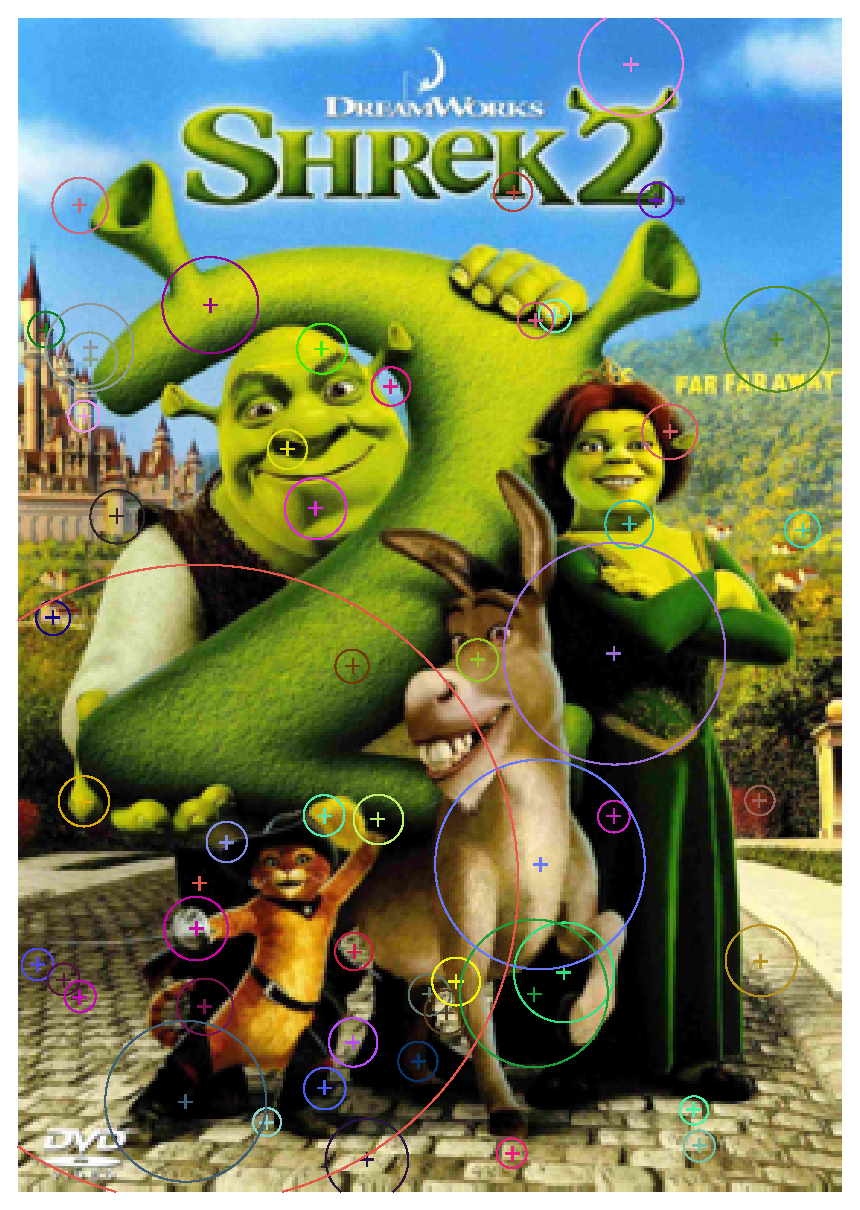
\includegraphics [width=4in]{debugScript_02.eps}
\begin{par}
test.png computed interest points
\end{par} \vspace{1em}
\begin{verbatim}
figure
plotInterestPoints(im2, locs2);
drawnow()
\end{verbatim}

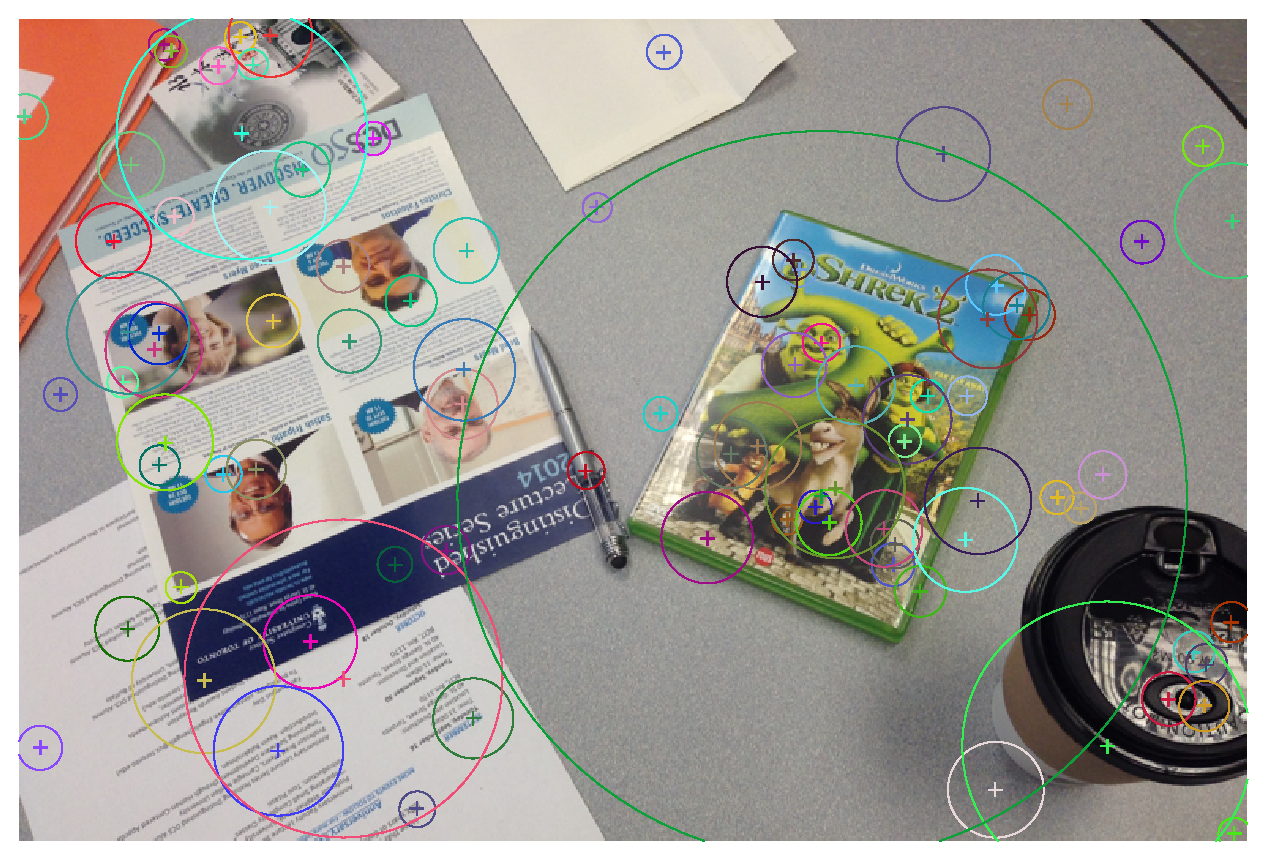
\includegraphics [width=4in]{debugScript_03.eps}
\begin{par}
Compute matches. See appendix for function code
\end{par} \vspace{1em}
\begin{verbatim}
matches = matchInterestPoints(desc1, desc2);
\end{verbatim}
\begin{par}
reference.png matched interest points
\end{par} \vspace{1em}
\begin{verbatim}
figure
plotInterestPoints(im1, locs1(matches(:,1),:), 1);
drawnow()
\end{verbatim}


\includegraphics [width=4in]{debugScript_04.eps}
\begin{par}
test.png matched interest points
\end{par} \vspace{1em}
\begin{verbatim}
figure
plotInterestPoints(im2, locs2(matches(:,2),:), 1);
drawnow()
\end{verbatim}

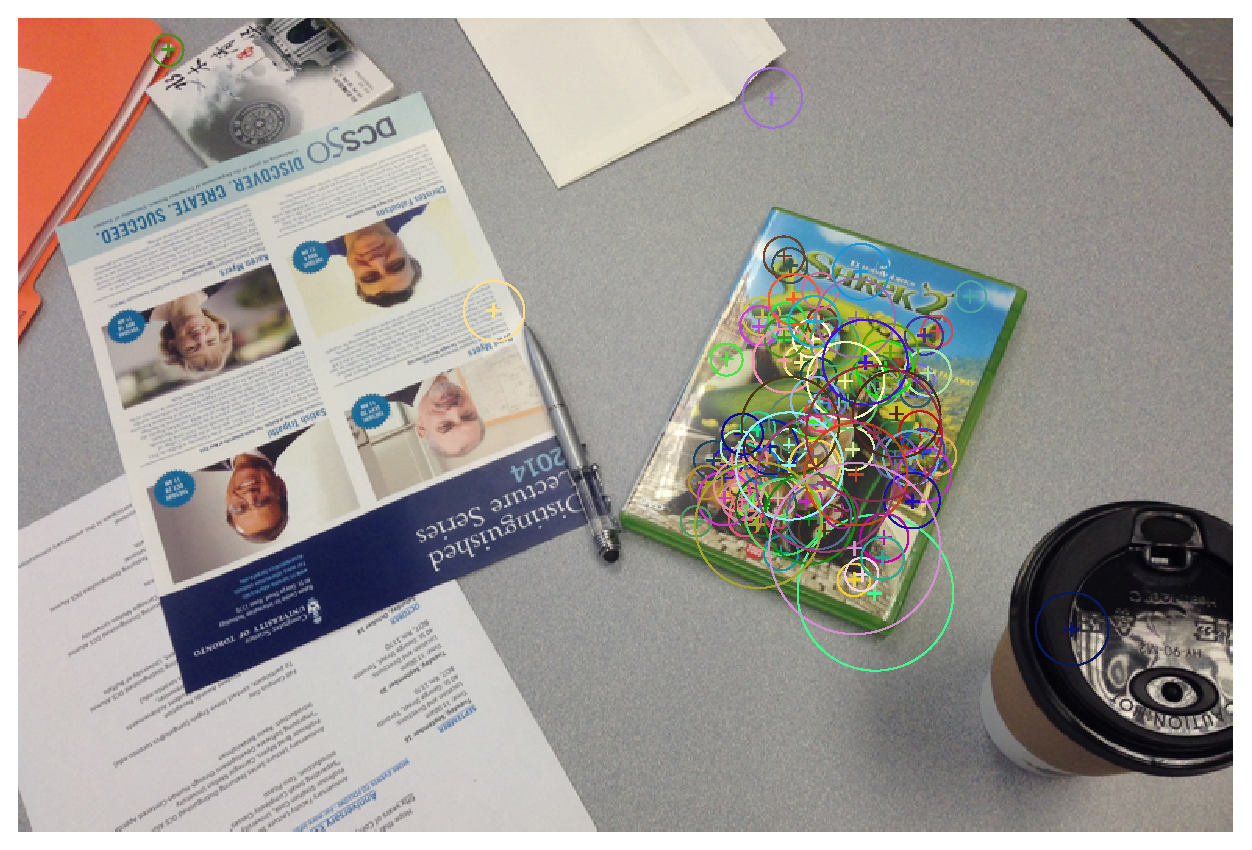
\includegraphics [width=4in]{debugScript_05.eps}
\begin{par}
note that colors of matched points in both images might be different and they do not indicate any correspondence
\end{par} \vspace{1em}
\begin{par}
Get best 3 matches (also included best 8 matches)
\end{par} \vspace{1em}
\begin{verbatim}
[B,I] = sort(matches(:,3)); %% sort by distances
top3 = matches(I(1:3),:);
top8 = matches(I(1:8),:);
\end{verbatim}
\begin{par}
Compute Affine transformation using top3, top8 matches as well as RANSAC
\end{par} \vspace{1em}
\begin{verbatim}
H3 = computeH(locs1(top3(:,1),1:2)', locs2(top3(:,2),1:2)');
H8 = computeH(locs1(top8(:,1),1:2)', locs2(top8(:,2),1:2)');
H = ransacH(matches, locs1, locs2);
\end{verbatim}
\begin{par}
See appendix for function codes
\end{par} \vspace{1em}
\begin{par}
Compute transformed corners
\end{par} \vspace{1em}
\begin{verbatim}
corners = [1,1,1;...
           1,size(im1,1),1;...
           size(im1,2),size(im1,1),1;...1
           size(im1,2),1,1;];
corners3 = (H3*corners')';
corners8 = (H8*corners')';
cornersR = (H*corners')';
\end{verbatim}
\begin{par}
Visualize transormation using top3 matches
\end{par} \vspace{1em}
\begin{verbatim}
figure
x = corners3(:,1);
y = corners3(:,2);
imshow(im2), hold on, fill(x,y,'r','FaceAlpha',0.3), hold off
drawnow()
\end{verbatim}

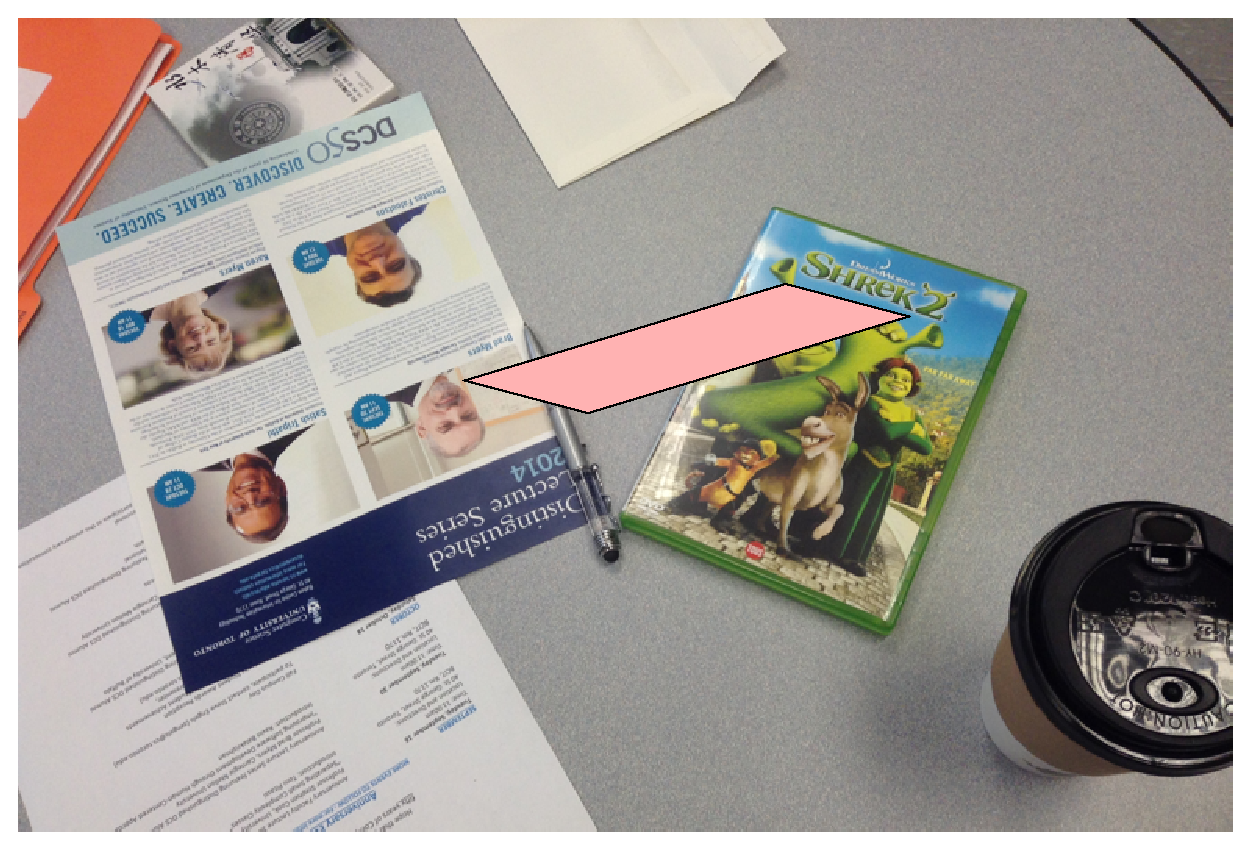
\includegraphics [width=4in]{debugScript_06.eps}
\begin{par}
Visualize transormation using top8 matches
\end{par} \vspace{1em}
\begin{verbatim}
figure
x = corners8(:,1);
y = corners8(:,2);
imshow(im2), hold on, fill(x,y,'r','FaceAlpha',0.3), hold off
drawnow()
\end{verbatim}

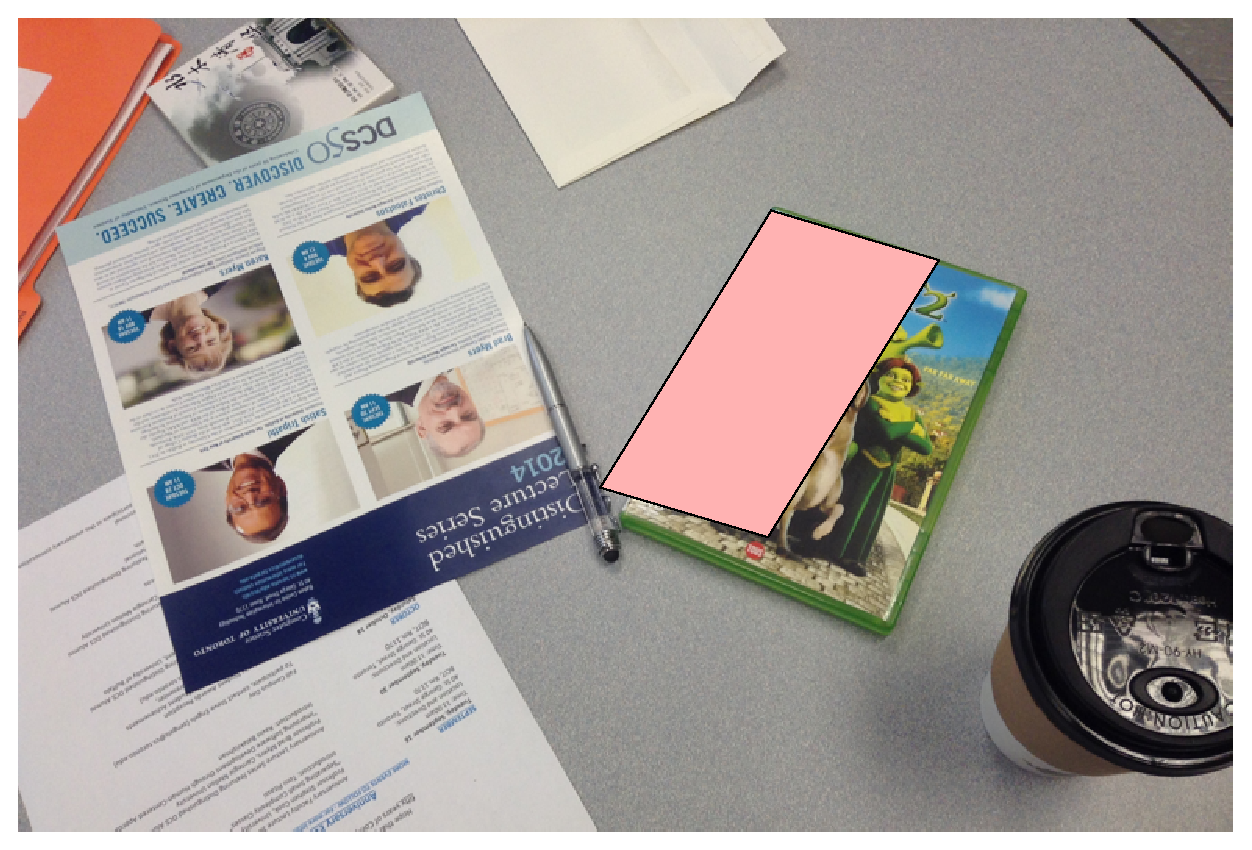
\includegraphics [width=4in]{debugScript_07.eps}
\begin{par}
Visualize transormation using RANSAC
\end{par} \vspace{1em}
\begin{verbatim}
figure
x = cornersR(:,1);
y = cornersR(:,2);
imshow(im2), hold on, fill(x,y,'r','FaceAlpha',0.3), hold off
drawnow()
\end{verbatim}

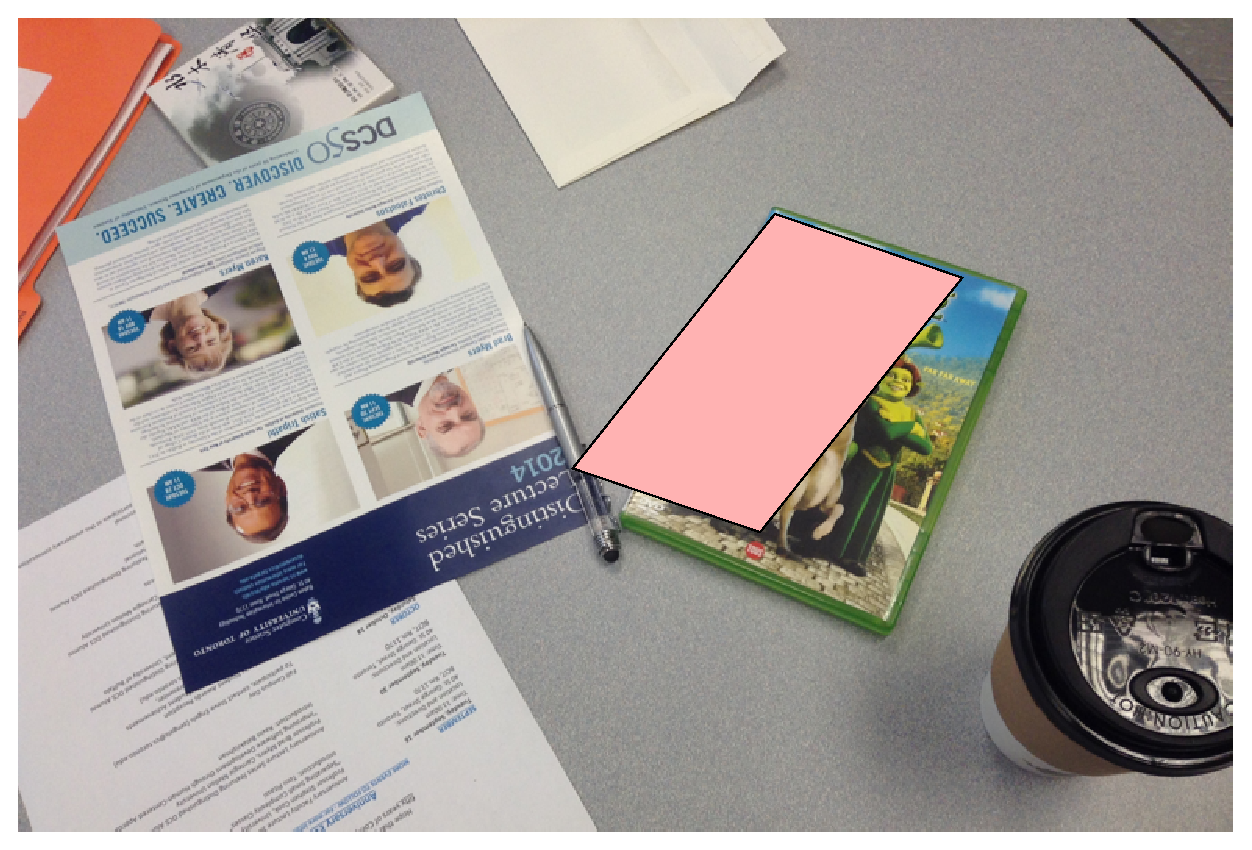
\includegraphics [width=4in]{debugScript_08.eps}


\subsection*{Appendix}

\begin{par}
All function definitions are here
\end{par} \vspace{1em}


\subsection*{function H2to1 = computeH(p1,p2)}

\begin{verbatim}
% function H2to1 = computeH(p1,p2)
% INPUTS:
% p1 and p2 - Each are size (2 x N) matrices of corresponding (x, y)'
%             coordinates between two images
%
% OUTPUTS:
% H2to1 - a 3 x 3 matrix encoding the homography that best matches the linear
%         equation
% p1 = p1';
% p2 = p2';
% A = [];
% for i = 1:size(p1,1)
%     x1 = p1(i,1);
%     x2 = p2(i,1);
%     y1 = p1(i,2);
%     y2 = p2(i,2);
%
%     A = vertcat(A,[-x1, -y1, -1, 0, 0, 0, x2*x1, x2*y1, x2]);
%     A = vertcat(A,[0, 0, 0, -x1, -y1, -1, y2*x1, y2*y1, y2]);
% end
% [V,~] = eig(A'*A);
% h = V(:,1);
% h = h/(h(end));
% H2to1 = reshape(h,[3,3])';
\end{verbatim}


\subsection*{function H = computeHessian(I)}

\begin{verbatim}
% function H = computeHessian(I)
% [ix,iy] = gradient(I);
% [H.ixx, H.ixy] = gradient(ix);
% [H.iyx, H.iyy] = gradient(iy);
% end
\end{verbatim}


\subsection*{function PrincipalCurvature = computePrincipalCurvature(DoGPyramid)}

\begin{verbatim}
% function PrincipalCurvature = computePrincipalCurvature(DoGPyramid)
%%Edge Suppression
% Takes in DoGPyramid generated in createDoGPyramid and returns
% PrincipalCurvature,a matrix of the same size where each point contains the
% curvature ratio R for the corre-sponding point in the DoG pyramid
%
% INPUTS
% DoG Pyramid - size (size(im), numel(levels) - 1) matrix of the DoG pyramid
%
% OUTPUTS
% PrincipalCurvature - size (size(im), numel(levels) - 1) matrix where each
%                      point contains the curvature ratio R for the
%                      corresponding point in the DoG pyramid
% PrincipalCurvature = zeros(size(DoGPyramid));
% for i = 1:size(DoGPyramid,3)
%     I = DoGPyramid(:,:,i);
%     H = computeHessian(I);
%     R = (tracefun(H).^2) ./ (detfun(H));
%     PrincipalCurvature(:,:,i) = R;
% end
% end
%
% function T = tracefun(H)
% T = H.ixx + H.iyy;
% end
%
% function D = detfun(H)
% D = ((H.ixx) .* (H.iyy)) - ((H.ixy) .* (H.iyx));
% end
\end{verbatim}


\subsection*{function [DoGPyramid, DoGLevels] = createDoGPyramid(GaussianPyramid, levels)}

\begin{verbatim}
% function [DoGPyramid, DoGLevels] = createDoGPyramid(GaussianPyramid, levels)
% Produces DoG Pyramid
% inputs
% Gaussian Pyramid - A matrix of grayscale images of size
%                    (size(im), numel(levels))
% levels      - the levels of the pyramid where the blur at each level is
%               outputs
% DoG Pyramid - size (size(im), numel(levels) - 1) matrix of the DoG pyramid
%               created by differencing the Gaussian Pyramid input
% L = numel(levels)-1;
% DoGPyramid = GaussianPyramid(:,:,1:end-1);
% for i = 1:L
%    DoGPyramid(:,:,i) = GaussianPyramid(:,:,i+1)-GaussianPyramid(:,:,i);
% end
% DoGLevels = levels(2:end);
%
% end
\end{verbatim}


\subsection*{function [GaussianPyramid] = createGaussianPyramid(im, sigma0, k, levels)}

\begin{verbatim}
% function [GaussianPyramid] = createGaussianPyramid(im, sigma0, k, levels)
% Produces Gaussian Pyramid
% inputs
% im - a grayscale image with range 0 to 1
% sigma0 - the standard deviation of the blur at level 0
% k - the multiplicative factor of sigma at each level, where sigma=sigma_0 k^l
% levels - the levels of the pyramid where the blur at each level is
% sigma=sigma0 k^l
% outputs
% A matrix of grayscale images of size (size(im),numel(levels))

% im = im2double(im);
% if size(im,3)==3
%     im= rgb2gray(im);
% end
%
% GaussianPyramid = zeros([size(im),length(levels)]);
% for i = 1:length(levels)
%     sigma_ = sigma0*k^levels(i);
%     h = fspecial('gaussian',floor(3*sigma_*2)+1,sigma_);
%     GaussianPyramid(:,:,i) = imfilter(im,h);
% end
\end{verbatim}


\subsection*{function displayPyramid(pyrmid)}

\begin{verbatim}
% function displayPyramid(pyrmid)
% inputs: pyrmid - R x C x L; R x C is the size of the input image; L is the number of levels in the pyramid.

% [nr, nc, nl]= size(pyrmid);
% im2show= zeros(nr, nc*nl);
%
% for il=1:nl
%     im2show(1:end,1+(il-1)*nc  :  il*nc) = pyrmid(:,:,il);
% end
%
% imshow(im2show,[]);
% title('Pyramid of image')
% end
\end{verbatim}


\subsection*{function [locsDoG, GaussianPyramid] = DoGdetector(im, sigma0, k, levels, th\_contrast, th\_r)}

\begin{verbatim}
% function [locsDoG, GaussianPyramid] = DoGdetector(im, sigma0, k, ...
%                                                 levels, th_contrast, th_r)
% DoGdetector
%  Putting it all together
%
%   Inputs          Description
% --------------------------------------------------------------------------
%   im              Grayscale image with range [0,1].
%
%   sigma0          Scale of the 0th image pyramid.
%
%   k               Pyramid Factor.  Suggest sqrt(2).
%
%   levels          Levels of pyramid to construct. Suggest -1:4.
%
%   th_contrast     DoG contrast threshold.  Suggest 0.03.
%
%   th_r            Principal Ratio threshold.  Suggest 12.
%
%   Outputs         Description
% --------------------------------------------------------------------------
%
%   locsDoG         N x 3 matrix where the DoG pyramid achieves a local extrema
%                   in both scale and space, and satisfies the two thresholds.
%
%   GaussianPyramid A matrix of grayscale images of size (size(im),numel(levels))
% GaussianPyramid = (createGaussianPyramid(im,...
%     sigma0,k, levels));
%
% [mypyrdog,L] = createDoGPyramid(GaussianPyramid, levels);
%
% pc = computePrincipalCurvature(mypyrdog);
%
% locsDoG = getLocalExtrema(mypyrdog, L, pc, th_contrast, th_r);
%
% end
\end{verbatim}


\subsection*{function locsDoG = getLocalExtrema(DoGPyramid, DoGLevels, PrincipalCurvature, th\_contrast, th\_r)}

\begin{verbatim}
% Detecting Extrema
% INPUTS
% DoG Pyramid - size (size(im), numel(levels) - 1) matrix of the DoG pyramid
% DoG Levels  - The levels of the pyramid where the blur at each level is
%               outputs
% PrincipalCurvature - size (size(im), numel(levels) - 1) matrix contains the
%                      curvature ratio R
% th_contrast - remove any point that is a local extremum but does not have a
%               DoG response magnitude above this threshold
% th_r        - remove any edge-like points that have too large a principal
%               curvature ratio
%
% OUTPUTS
% locsDoG - N x 3 matrix where the DoG pyramid achieves a local extrema in both
%           scale and space, and also satisfies the two thresholds.
% N = circshift(DoGPyramid,[-1, 0, 0]);
% NE = circshift(DoGPyramid,[-1, 1, 0]);
% E = circshift(DoGPyramid,[0, 1, 0]);
% SE = circshift(DoGPyramid,[1, 1, 0]);
% S = circshift(DoGPyramid,[1, 0, 0]);
% SW = circshift(DoGPyramid,[1, -1, 0]);
% W = circshift(DoGPyramid,[0, -1, 0]);
% NW = circshift(DoGPyramid,[-1, -1, 0]);
% Coarse = circshift(DoGPyramid,[0,0,1]);
% Fine = circshift(DoGPyramid,[0,0,-1]);
%
% locs = (DoGPyramid>=N)&(DoGPyramid>=NE)&(DoGPyramid>=E)&...
%     (DoGPyramid>=SE)&(DoGPyramid>=S)&(DoGPyramid>=SW)&...
%     (DoGPyramid>=W)&(DoGPyramid>=NW)&...
%     (DoGPyramid>=Coarse)&(DoGPyramid>=Fine);
% locs(:,:,1) = 0;
% locs(:,:,end) = 0;
% Xl = [];
% Yl = [];
% Dl = [];
% for i = 1:size(DoGPyramid,3)-2
%     iloc = locs(:,:,i+1);
%     D = DoGPyramid(:,:,i+1);
%     R = PrincipalCurvature(:,:,i+1);
%     iloc = iloc & (D>th_contrast);
%     iloc = iloc & (R<th_r);
%     [Yt,Xt] = find(iloc);
%     Xl = vertcat(Xl,Xt);
%     Yl = vertcat(Yl,Yt);
%     Dl = vertcat(Dl,DoGLevels(i+1)*ones(size(Xt)));
% end
% locsDoG = horzcat(Xl,Yl,Dl);
\end{verbatim}


\subsection*{function [matches] = matchInterestPoints(desc1, desc2, ratio)}

\begin{verbatim}
% function [matches] = briefMatch(desc1, desc2, ratio)
% Performs the descriptor matching
% inputs  : desc1 , desc2 - m1 x n and m2 x n matrix. m1 and m2 are the number of keypoints in image 1 and 2.
%						    n is the number of bits in the brief
% outputs : matches - p x 2 matrix. where the first column are indices
%									into desc1 and the second column are indices into desc2
%
% if nargin<3
%     ratio = .8;
% end
% D = dist2(desc1, desc2);
% ix = [];
% iy = [];
% d = [];
% for i = 1:size(D,1)
%    [B,I] = sort(D(i,:));
%    if (B(1)/B(2) > ratio), continue, end
%    ix(end+1) = i;
%    iy(end+1) = I(1);
%    d(end+1) = B(1);
% end
% matches = [ix', iy', d'];
% end
\end{verbatim}


\subsection*{function h = plotInterestPoints(im, locs, po)}

\begin{verbatim}
% im = image for interest points
% locs = locations of interest points, each row containing [x,y,scale]
% po = fraction of interests point to be drawn
% h = output handle for the plot
% h = imshow(im); hold on
% if ~exist('po','var')
%     po = 0.1;
% end
% s = max(size(im,1),size(im,2))/150;
% for  i = 1:size(locs,1);
%     if rand>po, continue, end
%     c = [rand rand rand];
%     try
%         rectangle('Position',...
%             [locs(i,1)-s*locs(i,3), locs(i,2)-s*locs(i,3), 2*s*locs(i,3), 2*s*locs(i,3)],...
%             'Curvature', [1 1],...
%             'EdgeColor', c);
%         scatter(locs(i,1),locs(i,2),[],c,'+')
%     catch
%         continue
%     end
%     pause(0.000000001)
% end
% hold off
% end
\end{verbatim}


\subsection*{function index = randIndex(maxIndex,len)}

\begin{verbatim}
% INDEX = RANDINDEX(MAXINDEX,LEN)
%   randomly, non-repeatedly select LEN integers from 1:MAXINDEX
%
% if len > maxIndex
% 	index = [];
% 	return
% end
%
% index = zeros(1,len);
% available = 1:maxIndex;
% rs = ceil(rand(1,len).*(maxIndex:-1:maxIndex-len+1));
% for p = 1:len
% 	while rs(p) == 0
% 		rs(p) = ceil(rand(1)*(maxIndex-p+1));
% 	end
% 	index(p) = available(rs(p));
% 	available(rs(p)) = [];
% end
%
\end{verbatim}


\subsection*{function [f] = ransac( x,y,ransacCoef,funcFindF,funcDist )}

\begin{verbatim}
%
% thInlrRatio = ransacCoef.thInlrRatio;
% thDist = ransacCoef.thDist;
% thInlr = round(thInlrRatio*size(x,2));
% inlrNum = zeros(1,ransacCoef.iterNum);
% fLib = cell(1,ransacCoef.iterNum);
% for p = 1:ransacCoef.iterNum
% 	sampleIdx = randIndex(size(x,2),max(thInlr,ransacCoef.minPtNum));
% 	f1 = funcFindF(x(:,sampleIdx),y(:,sampleIdx));
% 	dist = funcDist(f1,x,y);
% 	inlier1 = find(dist < thDist);
% 	inlrNum(p) = length(inlier1);
% 	if length(inlier1) < thInlr, continue; end
% 	fLib{p} = funcFindF(x(:,inlier1),y(:,inlier1));
% end
% [~,idx] = max(inlrNum);
% f = fLib{idx};
% end
\end{verbatim}


\subsection*{function bestH = ransacH(matches, locs1, locs2, nIter, tol)}

\begin{verbatim}
% INPUTS
% locs1 and locs2 - matrices specifying point locations in each of the images
% matches - matrix specifying matches between these two sets of point locations
% nIter - number of iterations to run RANSAC
% tol - tolerance value for considering a point to be an inlier
%
% OUTPUTS
% bestH - homography model with the most inliers found during RANSAC
% if ~exist('nIter','var')
%     nIter = 1000;
% end
% if ~exist('tol','var')
%     tol = 2;
% end
%
% p1 = locs1(matches(:,1),1:2);
% p2 = locs2(matches(:,2),1:2);
%
% coef.minPtNum = 16;
% coef.iterNum = nIter;
% coef.thDist = tol;
% coef.thInlrRatio = .1;
% bestH = ransac(p1',p2',coef,@computeH,@ptsDist);
% end
%
% function d = ptsDist(H,p1,p2)
% n = size(p1,2);
% p3 = H*[p1;ones(1,n)];
% p3 = p3(1:2,:)./repmat(p3(3,:),2,1);
% d = sqrt(sum((p2-p3).^2,1));
% end
\end{verbatim}



\end{document}
    
